\section{What 55B multimodal tokens buy}
\label{sec:vision-results}

\begin{figure}[t]
\centering
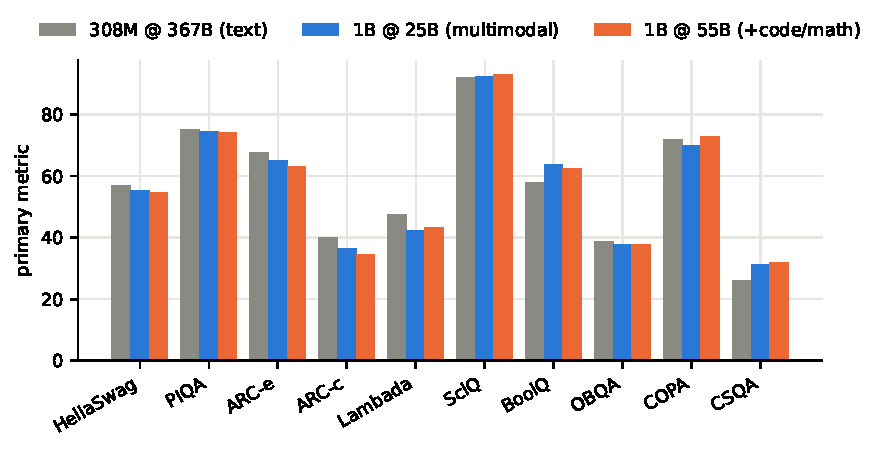
\includegraphics[width=\linewidth]{figures/vision_eval_bars.pdf}
\caption{Zero-shot primary metrics: the 308M text model at its full
367B-token budget versus the 1B multimodal model at 25B and 55B
tokens.}
\label{fig:vision-evals}
\end{figure}

\paragraph{Language holds at a fraction of the text budget.} With only
$\sim$12.8B of its supervised tokens on web text, the 25B-token trial
already beats the 337M 50B-token baseline of Part~I on every anchor,
and sits within a few points of the full 367B-token 308M campaign on
most (Figure~\ref{fig:vision-evals}); it is ahead outright on BoolQ
($+5.7$) and CommonsenseQA ($+5.2$). The continuation's added code and
mathematics leave this profile flat --- by design, its budget went
elsewhere: GSM8K (5-shot, full test set, greedy through the
incremental decoder) rises from 1.21\% to \textbf{3.18\%} exact-match,
versus 1.1\% for the 308M model at $6.7\times$ the text tokens.

\paragraph{Vision is grounded, not memorized.} On held-out probes the
final model counts objects, discriminates left from right, reads
synthetic and document text, identifies chart structure with values
read to within half a point, and localizes UI elements on screenshots
from shards the training pass never reached (a requested click lands
within 0.2\% in $x$). The trial model failed counting, mirrored
left/right, and refused synthetic OCR; thirty billion further tokens
repaired all three --- the classic small-VLM failure modes are budget
artifacts, not architectural ones.

\paragraph{Post-training transfers unchanged.} Because the 1B shares
Part~I's tokenizer, the entire post-training stack --- chat SFT and
GOLD distillation, including the \emph{same precomputed teacher
stores} --- applies verbatim. One day sufficed for four checkpoints:

\begin{center}
\begin{tabular}{lccc}
\toprule
checkpoint & IFEval mean & panel (32) & clean stops \\
\midrule
SFT-1 (dialogue-only mix) & 35.0 & 12 & 0/32 \\
\; + GOLD & 40.8 & 24 & 31/32 \\
SFT-2 (instruction-dense mix) & \textbf{55.3} & 23 & 32/32 \\
\; + GOLD & 48.8 & \textbf{27} & 32/32 \\
\midrule
308M best (Part I, GOLD) & 51.0 & --- & --- \\
\bottomrule
\end{tabular}
\end{center}

The instruction-dense second mix at a bolder learning rate is worth
$+20.3$ IFEval points over the first --- past every Part~I checkpoint
--- and distillation on top trades 6.5 of those points for the best
answer quality of the project (27/32), the teacher's discursive style
partially overwriting strict-format obedience. Constraint-following
tracks instruction-dense exposure; answer quality tracks the teacher:
the two live on a measurable frontier, and both frontier points belong
to the 1B.

\paragraph{Limitations.} GSM8K remains near-floor in absolute terms;
fine-grained visual categories and blocky synthetic text remain
brittle; instruction obedience at the strictest level trails what 367B
text tokens buy. Each gap moved monotonically with tokens in these
two campaigns, which is the scaling argument in its plainest form.
